\problem{}

\par Execute the Ford-Fulkerson algorithm on the flow network shown below. Display the residual network after each flow update and determine the maximum flow at the end. During each iteration, choose the lexicographically smallest available augmenting path. For example, if two augmenting paths are \( s \rightarrow 2 \rightarrow t \) and \( s \rightarrow 3 \rightarrow t \), select \( s \rightarrow 2 \rightarrow t \) since it is lexicographically smaller. Likewise, if the paths \( s \rightarrow 3 \rightarrow t \) and \( s \rightarrow 2 \rightarrow 4 \rightarrow t \) are available,  choose \( s \rightarrow 2 \rightarrow 4 \rightarrow t \). Moreover, if all compared vertices coincide up to the end of the shorter path, the shorter prefix path is considered smaller. For example, between \( s \rightarrow 1 \rightarrow t \) and \( s \rightarrow 1 \rightarrow 4 \rightarrow t \), select \( s \rightarrow 1 \rightarrow t \).

\medskip

\begin{figure}[h]
    \centering
    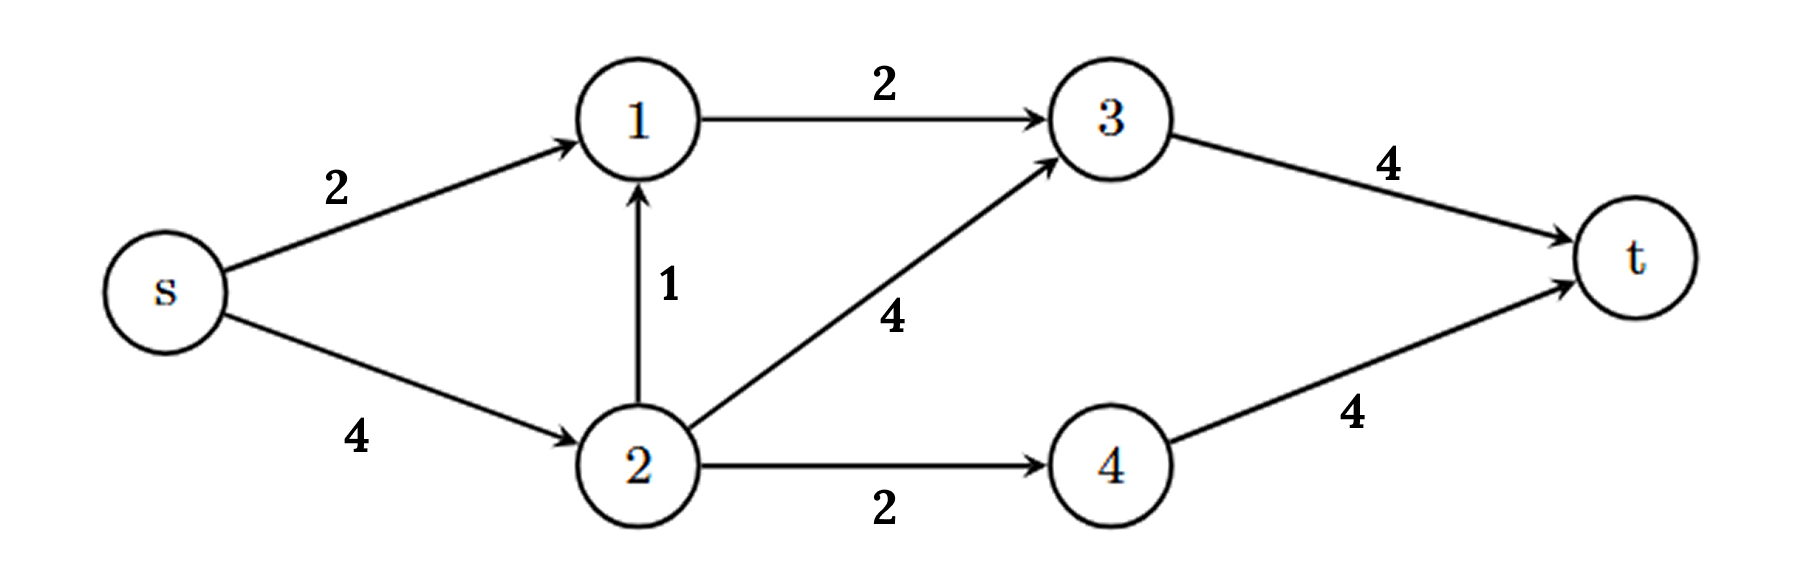
\includegraphics[width=\linewidth]{figure/Maximum Flow.png}
    
    \label{fig:enter-label}
\end{figure}

\noindent \textbf{Solution}:

Step1: the augmenting path is s → 1 → 3 → t. The capacity of this
path is min(2,2,4)=2.

\begin{figure}[h]
    \centering
    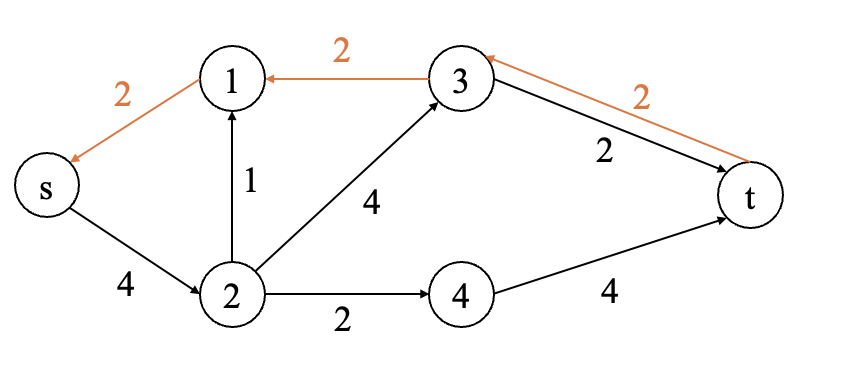
\includegraphics[width=\linewidth]{figure/1761143657899.png}
    
    
\end{figure}


Step2: the augmenting path is s → 2 → 3 → t. The capacity of this
path is min(4,4,2)=2.


\begin{figure}[h]
    \centering
    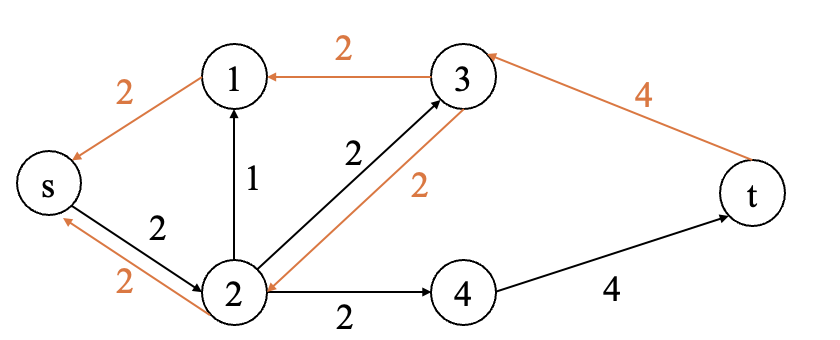
\includegraphics[width=\linewidth]{figure/1761143717944.png}
    
    
\end{figure}


Step3: the augmenting path is s → 2 → 4 → t. The capacity of this
path is min(2,2,4)=2.

\begin{figure}[h]
    \centering
    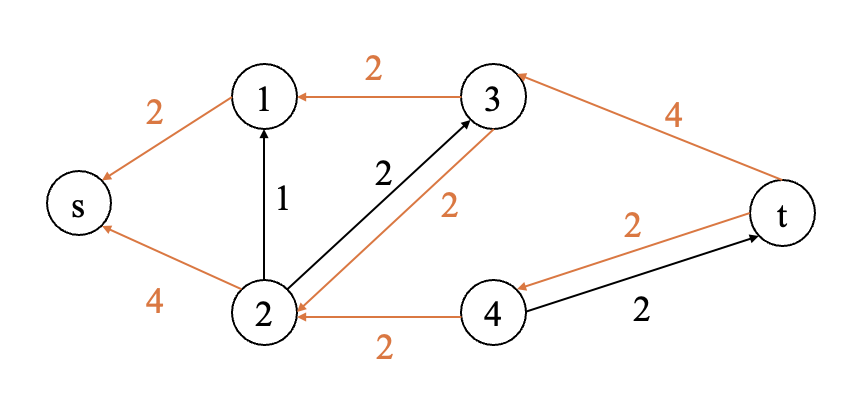
\includegraphics[width=\linewidth]{figure/1761143780498.png}
    
    
\end{figure}


The final maximum flow = 6
\newpage